%%==============================================================
%% Modelo de TCC para o curso de Sistemas de Informação
%% da Universidade Federal de Viçosa - Campus de Rio Paranaíba
%% Autor: Rodrigo Smarzaro (smarzaro@ufv.br)
%% Última versão Agosto/2021
%% Arquivo em formato UTF-8
%% Compilar com pdftex e biber
%% Precisa do arquivo abntex2-UFV.sty
%%==============================================================

\documentclass[
    % -- opções da classe memoir --
    12pt,                   % tamanho da fonte
    openright,              % capítulos começam em página ímpar (insere página vazia caso preciso)
    oneside,                % para impressão só no anverso. Oposto a twoside
    a4paper,                % tamanho do papel.
    % -- opções do pacote abntex2 --
    % chapter=TITLE,        % Títulos em maiúsculas
    sumario=tradicional,    % Sumário padrão memoir 
    % -- opções do pacote babel --
    english,                % idioma adicional para hifenização
    brazil,                 % idioma principal do documento
    ]{abntex2}

% Pacotes fundamentais
\usepackage{abntex2-UFV}        % Personalização para a Universidade Federal de Viçosa
\usepackage{lmodern}            % Usa a fonte Latin Modern
\usepackage[T1]{fontenc}        % Seleção de códigos de fonte de saída
\usepackage[utf8]{inputenc}        % Codificação do documento (conversão automática dos acentos)
\usepackage{indentfirst}        % Indenta o primeiro parágrafo de cada seção.
\usepackage{graphicx}            % Inclusão de gráficos
\usepackage{booktabs}           % \toprule, \midrule e \bottomrule para tabelas
\usepackage{csquotes}
\usepackage[final]{microtype} 			% para melhorias de justificação
\usepackage{hyphenat}




% Sistema autor-data com títulos nas referências em negrito
%\usepackage[alf,abnt-emphasize=bf]{abntex2cite}

% uso do biblatex, mais flexível e moderno
\usepackage[backend=biber,
            style=abnt,
            uniquename=init,
            giveninits,
            repeatfields,
            justify,
            noslsn]{biblatex}

\usepackage{xurl}
\urlstyle{same}

\addbibresource{referencias.bib}


%\PassOptionsToPackage{hyphens}{url}\usepackage{hyperref}
%\usepackage{url}
% permitir quebra de linha em URLs
%\makeatletter
%\g@addto@macro{\UrlBreaks}{\UrlOrds}
%\makeatother

\setlength\bibparsep{10pt}

% ---
% CONFIGURAÇÕES DE PACOTES
% ---

% Informações de dados para CAPA e FOLHA DE ROSTO
\titulo{Geração de Explicações de Código Baseadas em Inteligência Artificial com Foco na Identificação de Pontos Críticos e Alinhamento à Regra de Negócio para Programadores com Deficiência Visual}
\autor{João Pedro Silva Coelho}
\local{Rio Paranaíba}
\data{2026}
\orientador{Adriana Zanella Martinhago}    % redefinido no abntex2-UFV para aceitar Instituição (default = UFV-CRP)
%\coorientador{Nome do Coorientador}
\instituicao{Universidade Federal de Viçosa}

\campus{\emph{Campus} Rio Paranaíba}      % pacote abntex2-UFV
\curso{Sistemas de Informação}               % pacote abntex2-UFV
\membrobancaA{Membro da Banca A}             % pacote abntex2-UFV default = UFV-CRP
\membrobancaB{Membro da Banca B}       % pacote abntex2-UFV default = UFV-CRP
\databanca{\today}                           % pacote abntex2-UFV

% O preambulo deve conter o tipo do trabalho, o objetivo,
% o nome da instituição e a área de concentração
\preambulo{Monografia apresentada à Universidade Federal de Viçosa, como parte das exigências para a a aprovação na disciplina Trabalho de Conclusão de Curso I}
% ---

% ---
% Configurações de aparência do PDF final

% informações para o arquivo pdf de saída
% Interessante alterar a cor dos links para preto(black)
% na versão final para imprimir
\makeatletter
\hypersetup{
        % metadados
        pdftitle={\@title},
        pdfauthor={\@author},
        pdfsubject={\imprimirpreambulo},
        pdfcreator={LaTeX with abnTeX2},
        colorlinks=true,   % false: links em frame; true: links coloridos
        linkcolor=black,   % cor dos links no documento
        citecolor=blue,    % cor dos links para a bibliografia
        filecolor=magenta, % cor dos links para arquivos
        urlcolor=blue,     % cor dos links para sites
        bookmarksdepth=4   % profundidade do sumário do PDF
}
\makeatother
% ---

\begin{document}
% Retira espaço extra obsoleto entre as frases.
\frenchspacing

% ----------------------------------------------------------
% ELEMENTOS PRÉ-TEXTUAIS
% ----------------------------------------------------------
\pretextual

% Capa
\imprimircapa

% Folha de rosto
\imprimirfolhaderosto
% ---

% Inserir folha de aprovação
% \imprimirfolhadeaprovacao

% Dedicatória
% \begin{dedicatoria}
%    \vspace*{\fill}
%    \centering
%    \noindent
%    \textit{Texto qualquer da dedicatória}
%    \vspace*{\fill}
% \end{dedicatoria}
% ---

% Agradecimentos
% \begin{agradecimentos}
% %Insira o texto de agradecimentos aqui
% \end{agradecimentos}
% ---

% Epígrafe
% \begin{epigrafe}
%     \vspace*{\fill}
%     \begin{flushright}
%         \textit{``Word? nunca mais.''\\
%         (Qualquer usuário de \LaTeX)}
%     \end{flushright}
% \end{epigrafe}
% ---

% RESUMOS

% resumo em português
\begin{resumo}
 \noindent
 %Insira o resumo aqui
 A programação envolve processos cognitivos complexos, especialmente no que se refere à compreensão da lógica e das regras de negócio presentes no código-fonte. Para desenvolvedores com deficiência visual, esses desafios são intensificados devido às limitações das tecnologias assistivas, como leitores de tela, que oferecem uma leitura linear e com baixo nível de contextualização. Embora avanços recentes em Inteligência Artificial tenham ampliado as possibilidades de geração e explicação de código, essas soluções ainda não são projetadas considerando aspectos de acessibilidade ou a identificação de elementos semanticamente relevantes. Este trabalho propõe uma ferramenta baseada em Inteligência Artificial para a geração de explicações estruturadas de código, com foco na identificação de pontos críticos e no alinhamento à regra de negócio. A abordagem visa melhorar a compreensão do código por meio de descrições contextuais e semanticamente orientadas, adaptadas para acessibilidade.
 \vspace{\onelineskip}

 \noindent
 \textbf{Palavras-chaves}: Acessibilidade, Inteligência Artificial, Compreensão de Código
\end{resumo}

% resumo em inglês
\begin{resumo}[Abstract]
\begin{otherlanguage*}{english}
  \noindent
  %Insira o abstract aqui
  Programming involves complex cognitive processes, particularly with regard to understanding the logic and business rules embedded in source code. For developers with visual impairments, these challenges are intensified due to the limitations of assistive technologies such as screen readers, which provide a linear reading experience with limited contextualization. Although recent advances in Artificial Intelligence have expanded the possibilities for code generation and explanation, these solutions are generally not designed with accessibility considerations or the identification of semantically relevant elements in mind. This work proposes an Artificial Intelligence-based tool for generating structured code explanations, focusing on the identification of critical points and alignment with business rules. The proposed approach aims to improve code comprehension through contextual and semantically oriented descriptions adapted for accessibility.
  \vspace{\onelineskip}

  \noindent
  \textbf{Key-words}: Accessibility, Artificial Intelligence, Code Comprehension
 \end{otherlanguage*}
\end{resumo}

% inserir lista de ilustrações
\pdfbookmark[0]{\listfigurename}{lof}
\listoffigures*
\cleardoublepage
% ---

% inserir lista de tabelas
% \pdfbookmark[0]{\listtablename}{lot}
% \listoftables*
\cleardoublepage
% ---

% Lista de siglas e abreviaturas (opcional)
% sintaxe: \item [sigla] Descrição da sigla

%\begin{siglas}
%\item[ABNT] Absurdas Normas Técnicas
%\item[UFV] Universidade Federal de Viçosa
%\item[CRP] \emph{Campus} de Rio Paranaíba
%\end{siglas}

% Lista de símbolos (opcional)
% sintaxe: \item [simbolo] Descrição do símbolo

%\begin{simbolos}
%\item[$\infty$ ] Infinito
%\end{simbolos}

% inserir o sumario
\pdfbookmark[0]{\contentsname}{toc}
\tableofcontents*
\cleardoublepage
% ---

% ----------------------------------------------------------
% ELEMENTOS TEXTUAIS
% ----------------------------------------------------------
\textual

%Modifique a estrutura dos capítulos e seções de acordo com a necessidade do seu trabalho
\chapter{Introdução}\label{sec:introducao}
% Alguns links interessantes para se trabalhar com a classe abn\TeX\ e \LaTeX\ em geral\footnote{E também para usar alguns comandos de citação como exemplo}:
A Tecnologia da Informação ocupa um papel cada vez mais relevante na sociedade contemporânea, tornando o desenvolvimento de software uma atividade estratégica em diversos contextos, onde nesse cenário, segundo \textcite{acad54431201}, as pesquisas recentes têm investigado formas de ampliar a acessibilidade e promover a inclusão de pessoas com deficiência visual na programação e nos ambientes de desenvolvimento. Estudos como os de \textcite{latinoware20457} e \textcite{acad54431201} evidenciam que a compreensão do código representa um dos principais desafios enfrentados por programadores, especialmente em cenários que envolvem sistemas complexos e regras de negócio elaboradas, demandando elevado esforço cognitivo para interpretar a lógica implementada.

No contexto da acessibilidade, \textcite{latinoware20457}, ao investigarem a experiência de pessoas cegas em ambientes de desenvolvimento de software, identificaram que compreender e navegar pelo código-fonte representa uma das principais dificuldades enfrentadas durante a programação. Esses resultados reforçam a importância de soluções que auxiliem não apenas na edição do código, mas também em sua interpretação e entendimento contextual. As evidências apresentadas pelos autores fundamentam a proposta deste trabalho, que busca oferecer explicações estruturadas e semanticamente orientadas para facilitar a compreensão da lógica implementada e das regras de negócio.

Para programadores com deficiência visual, essas dificuldades tornam-se ainda mais significativas devido às limitações das tecnologias assistivas atualmente utilizadas. Ferramentas como leitores de tela, embora fundamentais para a acessibilidade digital, realizam predominantemente uma leitura linear do código, dificultando a percepção estrutural, a identificação de elementos críticos e a compreensão contextual da lógica implementada. \textcite{acad54431201} demonstram que tais limitações aumentam o esforço necessário para interpretar programas e compreender sua organização, impactando diretamente o processo de desenvolvimento de software.

Em resposta a essa demanda, a ferramenta proposta neste trabalho pretende gerar explicações contextualizadas que destaquem elementos relevantes e auxiliem desenvolvedores com deficiência visual na construção do entendimento semântico do sistema.

Paralelamente, o avanço recente da Inteligência Artificial, especialmente por meio de modelos capazes de compreender e gerar código-fonte, tem transformado significativamente a forma como desenvolvedores interagem com ambientes de programação. Ferramentas baseadas em Inteligência Artificial vêm sendo utilizadas para geração automática de código, explicação de funções, identificação de erros e apoio à documentação. \textcite{latinoware34224} exploram a aplicação dessas tecnologias para ampliar a acessibilidade e a produtividade de programadores cegos, identificando oportunidades relevantes para o uso de recursos inteligentes no apoio ao desenvolvimento.

Além disso, estudos relacionados à acessibilidade na programação demonstram que grande parte das soluções existentes concentra-se na adaptação de interfaces e no suporte ao uso de ambientes de desenvolvimento por pessoas com deficiência visual. \textcite{latinoware37693}, por exemplo, propõem diretrizes de acessibilidade para ambientes de desenvolvimento integrado, enquanto \textcite{latinoware40920} apresentam uma ferramenta voltada à estruturação acessível de código para programadores cegos ou com baixa visão. Apesar dessas contribuições, permanece uma lacuna no uso de recursos capazes de oferecer suporte à compreensão contextual da lógica implementada e das regras de negócio presentes no código.

Essa lacuna constitui uma das principais motivações deste trabalho. A ferramenta proposta busca integrar Inteligência Artificial e acessibilidade para produzir explicações semanticamente orientadas, complementando as iniciativas existentes e oferecendo suporte específico à compreensão de código-fonte por desenvolvedores com deficiência visual.
% \begin{alineas}
%   \item Informações da classe Abn\TeX : \textcite{abntex2classe,manualUFV}
%   \item Ajustes nas citações e referências: \textcite{biblatex}
%   \item Classe memoir (base do Abn\TeX\ ): \textapud{memoir}{abntex2classe}
%   \item Livros interessantes sobre \LaTeX: \cite{Dongen2012,LeslieLamport90,FrankMittelbach111,Dongen2012}
%   \item Distribuição \LaTeX\ para windows: \url{https://miktex.org/}
%   \item Editor \LaTeX\ gratuito: \url{http://texstudio.sourceforge.net/}
%   \item Gerenciador de arquivos \texttt{.bib}: \url{http://www.jabref.org/}
%   \item Gerenciador de artigos: \url{https://www.mendeley.com/}
%   \item Exemplo de Tabela: Veja \autoref{tab:cronograma}
%   \item Manual de Normas da UFV: \textcite{manualUFV}
% \end{alineas}

\section{Objetivos}\label{sec:objetivos}

\subsection{Objetivos Geral}

Identificar os principais desafios enfrentados por programadores com deficiência visual e as oportunidades de aplicação da Inteligência Artificial para apoiar a compreensão de código-fonte e regras de negócio.

\subsection{Objetivos Específicos}

\begin{itemize} 
  \item Realizar revisão e análise da literatura sobre acessibilidade, tecnologias assistivas e Inteligência Artificial aplicada à compreensão de código-fonte. 
  \item Definir os requisitos funcionais, não funcionais e os critérios para identificação de pontos críticos no código-fonte. 
  \item Definição de uma estrutura de explicação acessível compatível com leitores de tela e alinhada à compreensão de regras de negócio. 
  \item Desenvolver um protótipo capaz de processar código-fonte, identificar pontos críticos e gerar explicações por meio de Inteligência Artificial. 
  \item Validar tecnicamente o protótipo quanto à sua integração com leitores de tela e à conformidade com diretrizes de acessibilidade. 
\end{itemize}


\chapter{Referencial Teórico} 

O referencial teórico deste trabalho está fundamentado em estudos relacionados à acessibilidade computacional, programação para pessoas com deficiência visual, compreensão de código-fonte e aplicações de Inteligência Artificial na Engenharia de Software. A integração desses temas permite compreender os desafios enfrentados por programadores com deficiência visual e identificar oportunidades para o desenvolvimento de soluções mais acessíveis e semanticamente orientadas.

\section{Acessibilidade na programação}\label{sec:AcessComputacao}

A acessibilidade na computação tem como objetivo garantir que sistemas, ferramentas e tecnologias possam ser utilizados de forma autônoma e eficiente por diferentes perfis de usuários, incluindo pessoas com deficiência. No contexto da Engenharia de Software, esse conceito vai além da acessibilidade de aplicações destinadas ao usuário final, abrangendo também os ambientes e ferramentas empregados durante o processo de desenvolvimento \cite{latinoware37693}.

O crescimento da participação de pessoas com deficiência na área de tecnologia evidencia a necessidade de que ambientes de programação sejam concebidos de maneira inclusiva. Entretanto, muitas ferramentas de desenvolvimento ainda apresentam barreiras relacionadas à navegação, à organização das informações e à interação com tecnologias assistivas, dificultando a realização de tarefas cotidianas por desenvolvedores com deficiência visual \cite{latinoware20457}.

As diretrizes WCAG (\textit{Web Content Accessibility Guidelines}) estabelecem princípios fundamentais para o desenvolvimento de interfaces acessíveis, baseando-se nos pilares de perceptibilidade, operabilidade, compreensibilidade e robustez. Embora tenham sido originalmente propostas para aplicações web, diversos estudos apontam que seus princípios podem ser estendidos para ambientes de desenvolvimento integrado e outras ferramentas utilizadas por programadores, contribuindo para uma experiência mais inclusiva \cite{latinoware6969}.

No contexto específico da programação, a acessibilidade envolve garantir que editores de código, depuradores, navegadores de arquivos e demais componentes das IDEs possam ser utilizados de maneira eficiente por pessoas que dependem de leitores de tela ou outras tecnologias assistivas. Para isso, é fundamental que informações estruturais, mensagens do sistema e elementos da interface sejam corretamente disponibilizados por meio das APIs de acessibilidade e organizados de forma consistente \cite{latinoware37693}.

\textcite{acad54431201,latinoware20457} apresentam que programadores com deficiência visual frequentemente enfrentam dificuldades para compreender a estrutura global do código-fonte, localizar regras de negócio e navegar entre diferentes componentes do sistema. Essas limitações não decorrem apenas da complexidade inerente ao desenvolvimento de software, mas também das restrições impostas pelas ferramentas atualmente disponíveis, que muitas vezes privilegiam elementos visuais em detrimento de representações acessíveis. Dessa forma, promover acessibilidade na programação não significa apenas adaptar interfaces existentes, mas também desenvolver soluções capazes de apresentar informações de maneira estruturada e semanticamente significativa. Essa perspectiva abre espaço para o emprego de tecnologias como a Inteligência Artificial na geração de explicações acessíveis e no suporte à compreensão de código-fonte por programadores com deficiência visual, tema central desta pesquisa.

\section{Tecnologias Assistivas e Leitores de Tela}\label{sec:TrabRel}
  As tecnologias assistivas desempenham papel fundamental na promoção da acessibilidade digital para pessoas com deficiência visual. Entre essas tecnologias, os leitores de tela destacam-se como os principais mecanismos utilizados para interação com sistemas computacionais, ambientes de desenvolvimento e aplicações web \cite{latinoware20457}. 
  
  Leitores de tela são softwares responsáveis por interpretar informações exibidas na interface gráfica do sistema operacional e convertê-las em saída sonora ou tátil, permitindo que usuários com deficiência visual naveguem e interajam com aplicações digitais \cite{latinoware37693}. 
  
  Dentre os leitores de tela mais utilizados atualmente, destaca-se o NVDA \textit{(NonVisual Desktop Access)}, software gratuito e de código aberto amplamente adotado por usuários com deficiência visual \cite{latinoware20457}. 
  
  O funcionamento do NVDA baseia-se principalmente em navegação sequencial. O usuário interage com os elementos da interface por meio de atalhos de teclado, enquanto o leitor de tela anuncia informações relacionadas ao componente atualmente em foco. Em ambientes de programação, o software realiza a leitura linha a linha do código-fonte \cite{latinoware20457}. 
  
  Embora o NVDA represente uma ferramenta essencial para inclusão digital, estudos apontam limitações importantes no contexto da programação. A leitura predominantemente linear dificulta a compreensão estrutural do código, tornando mais complexa a identificação de relacionamentos entre funções, blocos condicionais e regras de negócio. Além disso, tarefas como navegação entre arquivos, interpretação de fluxos lógicos e identificação de pontos críticos exigem elevado esforço cognitivo por parte do usuário \cite{acad54431201}.  
  \begin{figure}[htbp]
    \centering
    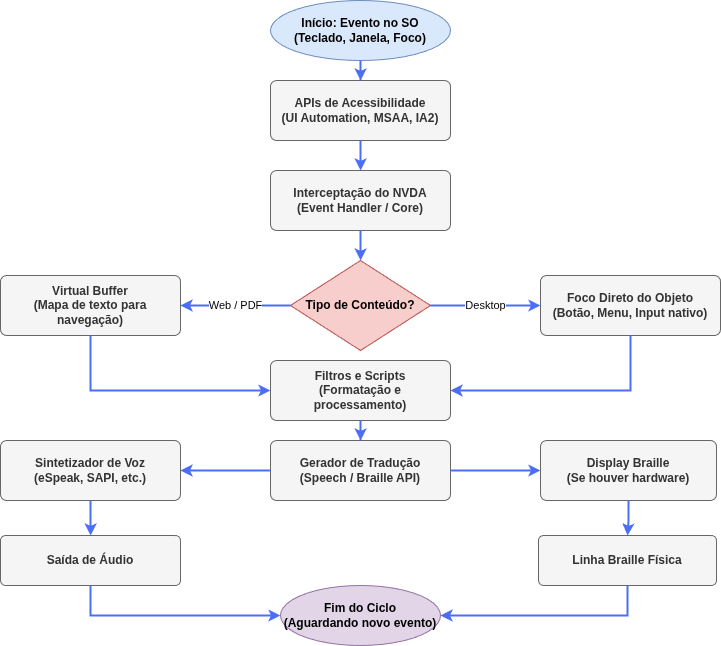
\includegraphics[width=.7\linewidth]{fluxograma_NVDA.png}
    \caption{Figura 1: Diagrama do ciclo de execução do leitor de tela NVDA, evidenciando a captura de eventos por APIs (MSAA, UIA, IA2), a divisão de processamento por tipo de conteúdo (\textit{Buffer Virtual } e Foco Direto) e as interfaces de saída de áudio e braille.}
    \legend{Fonte: Adaptada de \cite{latinoware6969}}
    \label{fig:my_label}
  \end{figure}
  

  A Figura 1 ilustra apresenta o funcionamento de um leitor de tela. O processo inicia com um evento no sistema operacional, como o pressionamento de uma tecla ou a mudança de foco, que é capturado pelas APIs de acessibilidade. Em seguida, o leitor de tela interpreta essas informações e identifica o tipo de conteúdo acessado, podendo utilizar um \textit{Virtual Buffer} para páginas web e documentos ou acessar diretamente os elementos da interface em aplicações desktop. Após o processamento e aplicação de filtros, as informações são convertidas para formatos acessíveis e apresentadas ao usuário por meio de um sintetizador de voz ou de um display Braille, quando disponível. Esse ciclo se repete continuamente à medida que novos eventos são gerados pelo sistema \cite{latinoware6969}. 

\section{Inteligência Artificial}\label{sec:IA}

A Inteligência Artificial (IA), destacada por \textcite{latinoware34224}, consiste em um campo da Ciência da Computação dedicado ao desenvolvimento de sistemas capazes de executar tarefas que, tradicionalmente, exigiriam inteligência humana, como aprendizado, reconhecimento de padrões, tomada de decisão e resolução de problemas. Nas últimas décadas, os avanços em capacidade computacional e disponibilidade de dados impulsionaram significativamente a evolução dessa área, possibilitando o desenvolvimento de modelos cada vez mais sofisticados e aplicáveis em diferentes domínios.

\textcite{latinoware34224} aporta que, entre as principais abordagens de IA, destacam-se o aprendizado de máquina (\textit{machine learning}), o aprendizado profundo (\textit{deep learning}) e os modelos de linguagem de grande porte (\textit{Large Language Models} -- LLMs). Essas técnicas permitem que sistemas sejam treinados a partir de grandes volumes de dados para reconhecer padrões, gerar conteúdo e realizar inferências de maneira automatizada, ampliando seu potencial de aplicação em atividades complexas.

Os recentes avanços em modelos generativos possibilitaram o desenvolvimento de ferramentas capazes de produzir textos, imagens e código-fonte com elevado grau de coerência. No contexto da programação, esses modelos passaram a compreender estruturas sintáticas e semânticas das linguagens de programação, permitindo não apenas gerar código, mas também resumir funcionalidades, explicar trechos específicos e auxiliar na documentação de sistemas \cite{latinoware34224}.

\subsection{Inteligência Artificial Aplicada à Engenharia de Software}\label{sec:IAES}

Na Engenharia de Software, a Inteligência Artificial tem sido empregada em atividades relacionadas à geração, análise, manutenção e compreensão de código-fonte. Ferramentas baseadas em IA passaram a integrar ambientes de desenvolvimento modernos, auxiliando programadores em tarefas como geração automática de código, documentação, identificação de erros e explicação de funções \cite{latinoware34224}.

Além da automação de tarefas de desenvolvimento apresentada por \textcite{latinoware34224}, pesquisas relacionadas à sumarização automática de código (\textit{code summarization}) demonstram que descrições semânticas e contextualizadas podem melhorar significativamente a compreensão do comportamento de sistemas. Essas técnicas permitem transformar estruturas técnicas em explicações orientadas à lógica funcional e às regras de negócio, reduzindo o esforço cognitivo necessário para interpretar códigos complexos.

Entretanto, apesar dos avanços observados, a maior parte das soluções atuais foi projetada com foco em produtividade geral, sem considerar requisitos específicos de acessibilidade. Em consequência, usuários que dependem de tecnologias assistivas, como leitores de tela, frequentemente recebem explicações genéricas ou pouco estruturadas, dificultando a compreensão do código-fonte \cite{latinoware34224}.

Nesse contexto, \textcite{latinoware34224} e \textcite{latinoware40920} destacam a aplicação da Inteligência Artificial para apoiar programadores com deficiência visual representa uma oportunidade relevante de pesquisa. A integração entre modelos generativos, identificação de pontos críticos do código e geração de explicações semanticamente estruturadas pode contribuir para reduzir barreiras de acessibilidade e facilitar a compreensão de regras de negócio em sistemas de software.


\section{Prototipação}\label{sec:Prototipacao}

A prototipação é uma técnica amplamente empregada no desenvolvimento de software para representar, de forma preliminar, as características e funcionalidades de um sistema antes de sua implementação definitiva. Segundo \textcite{latinoware7985}, seu principal objetivo é permitir a validação de requisitos, apoiar a comunicação entre as partes interessadas e identificar problemas de usabilidade ou inconsistências ainda nas fases iniciais do desenvolvimento.

Os protótipos podem variar quanto ao seu nível de detalhamento. Os chamados protótipos de baixa fidelidade consistem em representações simplificadas, como esboços ou modelos conceituais, utilizadas para explorar ideias e avaliar aspectos gerais da interface ou do fluxo de interação. Por outro lado, os protótipos de alta fidelidade apresentam maior grau de detalhamento visual e funcional, aproximando-se do comportamento esperado do sistema final e permitindo avaliações mais precisas por parte dos usuários \cite{latinoware7985}.

Além da classificação por fidelidade, a literatura também distingue diferentes estratégias de prototipação. Na prototipação descartável (\textit{throwaway prototyping}), o protótipo é desenvolvido apenas para compreender requisitos ou validar soluções específicas, sendo posteriormente descartado. Já na prototipação evolutiva (\textit{evolutionary prototyping}), o modelo inicial é progressivamente refinado até se tornar parte do sistema final, incorporando melhorias ao longo do processo de desenvolvimento \cite{latinoware7985}.

No contexto da Engenharia de Software,\textcite{latinoware7985} propõe a que prototipação desempenha um papel importante na redução de riscos e na melhoria da qualidade do produto, permitindo identificar problemas antes das etapas de implementação definitiva. Além disso, sua utilização favorece o alinhamento entre requisitos funcionais, necessidades dos usuários e soluções técnicas, contribuindo para o desenvolvimento de sistemas mais adequados ao contexto de uso.


\chapter{Trabalhos Relacionados}\label{sec:TrabRel}

O presente trabalho se insere em um contexto de crescente interesse na interseção entre Inteligência Artificial (IA), Engenharia de Software e Acessibilidade. Para contextualizar e fundamentar a proposta, foram analisados trabalhos relevantes que abordam desafios enfrentados por programadores com deficiência visual, o uso de modelos de linguagem pré-treinados para código e revisões sistemáticas sobre a aplicação de IA na Engenharia de Software. A seguir, são apresentados três trabalhos que se destacam por sua relevância e que estabelecem uma base para a compreensão e o desenvolvimento da ferramenta proposta.

\section{Inteligência Artificial e Acessibilidade: Uma Experiência de Inclusão para Programadores Cegos em Ambientes de Desenvolvimento}

\textcite{latinoware34224} exploram o uso de ferramentas de Inteligência Artificial para aumentar a acessibilidade e a produtividade no ensino de programação para estudantes cegos. A pesquisa avaliou desafios e sucessos em ambientes como \textit{VS Code} e \textit{Repl.it}, utilizando questionários e entrevistas com programadores cegos. Os resultados apontaram barreiras significativas, como dificuldades de navegação e limitações em leitores de tela, além de sugerir melhorias. Este estudo oferece lições valiosas para educadores que buscam replicar ou adaptar intervenções, incentivando o uso da IA para um ensino de programação mais inclusivo.

A identificação das barreiras e das estratégias de contorno utilizadas por programadores com deficiência visual serve como base para a definição dos requisitos da ferramenta proposta, que busca oferecer explicações estruturadas e alinhadas à regra de negócio, minimizando o esforço cognitivo e promovendo uma interação mais eficiente com o código-fonte. A experiência relatada por \textcite{latinoware34224} reforça a relevância de integrar IA para superar as limitações das tecnologias assistivas atuais.

\section{WAE - Web Accessibility Engine: Uma Ferramenta de Transpilação Acessível e Estruturada para Programadores Cegos ou de Baixa Visão}

\textcite{latinoware40920} apresentam o WAE \textit{(Web Accessibility Engine)}, uma ferramenta desenvolvida para facilitar a prototipação e o desenvolvimento de páginas web estáticas por programadores cegos ou com baixa visão. A pesquisa incluiu uma revisão da literatura que levou à escolha do paradigma de codificação acessível \textit{Grid Coding} e da linguagem YAML como bases para o projeto. A avaliação da acessibilidade das páginas geradas pelo WAE foi realizada utilizando o Avaliador e Simulador de Acessibilidade em Sítios (ASES), e os resultados indicaram que a maioria dos componentes criados pelo WAE atendeu a altos padrões de acessibilidade. Este estudo demonstra o potencial da ferramenta para contribuir significativamente para o desenvolvimento web inclusivo.

O artigo de \textcite{latinoware40920} é diretamente relevante para este trabalho, pois aborda a criação de ferramentas que promovem a acessibilidade no desenvolvimento de software por meio de paradigmas de codificação estruturados. A ênfase do WAE em uma abordagem acessível e estruturada para a criação de código web está alinhada ao objetivo deste trabalho de gerar explicações de código estruturadas e semanticamente orientadas. Além disso, a metodologia de avaliação da acessibilidade utilizada no WAE oferece subsídios para avaliar a efetividade da ferramenta proposta, garantindo que as explicações geradas sejam úteis para programadores com deficiência visual.

\section{Diretrizes de Acessibilidade em Ambientes de Desenvolvimento Integrado para Estudantes Cegos}

As diretrizes de acessibilidade propostas por \textcite{latinoware37693} para o projeto de Ambientes de Desenvolvimento Integrado (IDEs) voltadas para estudantes cegos, foi motivado pela constatação de que os IDEs tradicionais, por utilizarem elementos gráficos não totalmente acessíveis a leitores de tela, podem prejudicar a aprendizagem de programação por esse público. A metodologia empregou sete estágios, incluindo revisão de literatura, questionários, entrevistas e grupo focal, e os resultados confirmaram que as recomendações desenvolvidas são eficazes em apoiar o desenvolvimento de IDEs mais acessíveis.

\textcite{latinoware37693} oferece um arcabouço teórico e prático essencial para a presente pesquisa ao focar na especificação de diretrizes de acessibilidade para IDEs. A proposta desta pesquisa de desenvolver uma ferramenta para geração de explicações de código está diretamente alinhada à necessidade de tornar os ambientes de desenvolvimento mais inclusivos. As diretrizes apresentadas podem orientar o projeto e a implementação da ferramenta proposta, contribuindo para que as explicações sejam não apenas precisas, mas também acessíveis e integradas ao fluxo de trabalho de programadores com deficiência visual.



\chapter{Métodos}\label{sec:metodos}

A metodologia deste trabalho está estruturada para o desenvolvimento e avaliação de um protótipo conceitual de uma ferramenta baseada em Inteligência Artificial (IA) para a geração de explicações estruturadas de código-fonte. O foco principal é a identificação de pontos críticos e o alinhamento à regra de negócio, visando apoiar a compreensão de código por programadores com deficiência visual. A abordagem metodológica será guiada pelas lacunas e oportunidades identificadas em trabalhos relacionados, conforme detalhado a seguir.

\section{Revisão e Análise Preliminar}

Esta etapa inicial consiste na revisão aprofundada da literatura existente sobre acessibilidade na computação, desafios enfrentados por programadores com deficiência visual, tecnologias assistivas (especialmente leitores de tela) e aplicações de Inteligência Artificial na Engenharia de Software. O objetivo é consolidar o entendimento sobre o estado da arte e identificar lacunas de pesquisa que a presente proposta busca preencher. Artigos como o de \textcite{latinoware34224}, que explora o uso de IA para inclusão de programadores cegos, e \textcite{latinoware37693}, que propõe diretrizes de acessibilidade para IDEs, são cruciais para fundamentar a compreensão dos desafios e a necessidade de soluções inovadoras. A análise desses estudos permitirá uma compreensão mais aprofundada das limitações das ferramentas atuais para usuários com deficiência visual e das estratégias que podem ser adotadas para superá-las.

\section{Definição de Requisitos e Critérios}

Com base na revisão da literatura e nos objetivos específicos do trabalho, serão definidos os requisitos funcionais e não funcionais para a ferramenta proposta. Esta etapa incluirá:

Identificação dos desafios: Detalhamento dos principais obstáculos enfrentados por programadores com deficiência visual na compreensão de código-fonte. Análise das limitações das tecnologias assistivas: Avaliação das deficiências dos leitores de tela e outras tecnologias assistivas no contexto da interpretação de código.

Definição de critérios para pontos críticos: Estabelecimento de um conjunto de critérios para identificar e categorizar pontos críticos no código-fonte. Esta definição será informada pela necessidade de ir além da leitura linear, conforme sugerido pelos trabalhos que abordam as dificuldades de navegação e compreensão estrutural.

\section{Definição da Estratégia de Geração de Explicações}

Após o levantamento dos requisitos, será definida a estratégia utilizada pelo protótipo para produzir explicações sobre o código-fonte. Essa estratégia consistirá na elaboração de instruções \textit{(prompts)} para o modelo de Inteligência Artificial, especificando quais informações devem ser priorizadas e como elas devem ser organizadas na resposta.

As explicações serão estruturadas de forma hierárquica, iniciando por uma visão geral da finalidade do trecho analisado e, em seguida, detalhando seus principais componentes, como métodos, estruturas condicionais, laços de repetição e chamadas relevantes. Sempre que possível, a descrição também deverá relacionar esses elementos à regra de negócio implementada.

Para favorecer o uso com tecnologias assistivas, o formato das respostas evitará tabelas, símbolos excessivos e dependência de elementos exclusivamente visuais. As informações serão apresentadas em linguagem textual clara, segmentadas em tópicos e organizadas em uma sequência lógica, permitindo que leitores de tela realizem a leitura de maneira mais fluida e que o usuário possa localizar rapidamente as partes mais relevantes da explicação.


\section{Desenvolvimento do Protótipo Conceitual}

O protótipo terá como objetivo demonstrar a viabilidade da abordagem proposta e validar as ideias desenvolvidas nas etapas anteriores. Sua implementação será realizada integralmente em Python, consistindo em uma aplicação funcional capaz de receber o código-fonte como entrada, processá-lo, gerar explicações estruturadas e disponibilizá-las ao usuário por meio da integração com tecnologias assistivas.

Para isso, a análise estrutural do código-fonte será realizada por meio da biblioteca Tree-sitter do Python, responsável pela construção da Árvore Sintática Abstrata (AST), permitindo a identificação automatizada de pontos críticos, como condicionais aninhados, laços extensos e chamadas a dependências, por meio de regras de mapeamento sintático. A geração das explicações textualmente estruturadas será conduzida por um LLM, empregando-se primariamente a API do GPT-4o e, como alternativa local, o modelo Llama 3 executado via Ollama, ambos acessados por requisições HTTP e orientados por prompts que especificam a produção de descrições hierárquicas, em linguagem clara e alinhadas à regra de negócio.

O protótipo contará ainda com integração à biblioteca NVDA Controller Client, permitindo o envio das explicações diretamente ao leitor de telas NVDA e garantindo sua reprodução em áudio. Dessa forma, o sistema reunirá, em um único fluxo de execução implementado em Python, as etapas de extração da AST, análise estrutural do código, comunicação com o modelo de linguagem e disponibilização das explicações ao usuário, possibilitando a avaliação prática da viabilidade técnica da solução proposta.


\section{Validação Técnica e Conformidade com Diretrizes de Acessibilidade}

A validação do protótipo será conduzida por meio de estratégias técnicas e automatizadas, buscando verificar sua integração com tecnologias assistivas e sua aderência aos requisitos definidos ao longo do trabalho.

\subsection{Teste Automatizado com NVDA Controller Client}

Uma das estratégias de validação consiste na utilização da API \textit{NVDA Controller Client}, que permite que aplicações externas se comuniquem diretamente com o leitor de telas NVDA por meio do envio de comandos de fala ou braille. Essa funcionalidade será empregada para verificar se as explicações produzidas pelo protótipo podem ser corretamente transmitidas ao leitor de telas.

Para a realização do teste, será desenvolvido um script em Python responsável por:

\begin{enumerate}
  \item Carregar a biblioteca \texttt{nvdaControllerClient.dll}, compatível com o ambiente de execução
  \item Enviar as explicações geradas pelo protótipo ao NVDA
  \item Registrar os códigos de retorno e eventuais erros de comunicação durante a execução.
\end{enumerate}

Os testes serão executados em um ambiente controlado, com o NVDA em funcionamento, permitindo verificar a correta comunicação entre o protótipo e o leitor de telas e identificar possíveis falhas de integração.


\chapter{Resultados Esperados}\label{sec:resultEsperados}

Espera-se que este trabalho resulte em um protótipo conceitual capaz de analisar código-fonte e gerar explicações estruturadas em linguagem natural, destacando pontos críticos da implementação e relacionando-os, sempre que possível, à regra de negócio correspondente, de forma organizada e compatível com tecnologias assistivas como leitores de tela. Além do desenvolvimento do protótipo, espera-se identificar e sistematizar os principais desafios enfrentados por programadores com deficiência visual na compreensão de código, estabelecer requisitos e critérios para a geração de explicações acessíveis e demonstrar, por meio de validação técnica, a viabilidade da integração entre a solução proposta e o leitor de telas NVDA. Em conjunto, esses resultados têm o potencial de evidenciar a aplicabilidade da Inteligência Artificial como ferramenta de apoio à acessibilidade na Engenharia de Software e fornecer uma base para futuras pesquisas e soluções voltadas à inclusão de programadores com deficiência visual.


% \chapter{Conclusão}

% A presente trabalho propos uma ferramenta baseada em Inteligência Artificial para a geração de explicações estruturadas de código-fonte, com foco na identificação de pontos críticos e na contextualização da regra de negócio, visando apoiar programadores com deficiência visual durante atividades de compreensão de software. A motivação para essa proposta decorre das limitações identificadas na literatura em relação às tecnologias assistivas atualmente disponíveis, especialmente os leitores de tela, que apresentam dificuldades para transmitir de forma eficiente a estrutura e o contexto semântico do código-fonte.

% A revisão da literatura evidenciou que, embora os avanços recentes em Inteligência Artificial tenham ampliado significativamente as possibilidades de geração e interpretação automática de código, ainda existem poucas iniciativas voltadas especificamente às necessidades de acessibilidade de programadores com deficiência visual. Nesse contexto, este trabalho busca contribuir ao integrar conceitos de Inteligência Artificial, Engenharia de Software e acessibilidade em uma abordagem voltada à geração de explicações mais contextualizadas e compatíveis com tecnologias assistivas.

% Com base no levantamento bibliográfico, foram definidos requisitos para a ferramenta proposta e estabelecida uma estratégia para a geração de explicações utilizando modelos de linguagem de grande porte e técnicas de engenharia de prompts. Além disso, foi concebido um protótipo cuja arquitetura prevê a integração entre o modelo de IA e o leitor de telas NVDA, juntamente com uma estratégia de validação técnica baseada na API NVDA Controller Client para verificar a correta comunicação entre os componentes do sistema.

% Espera-se que a abordagem proposta demonstre o potencial da Inteligência Artificial para apoiar a compreensão de código-fonte por programadores com deficiência visual, fornecendo explicações que destaquem elementos relevantes da implementação e seu relacionamento com a lógica de negócio. Embora a efetividade da solução dependa de avaliações práticas com usuários, o trabalho estabelece uma base metodológica e tecnológica para o desenvolvimento de ferramentas mais acessíveis voltadas à programação.

% Como continuidade desta pesquisa, recomenda-se a realização de estudos com programadores com deficiência visual para avaliar a utilidade, a usabilidade e a efetividade das explicações geradas em cenários reais de desenvolvimento. Também são perspectivas futuras a personalização das explicações de acordo com o perfil e a experiência do usuário, o suporte a diferentes linguagens de programação e a integração da solução a ambientes de desenvolvimento amplamente utilizados, ampliando seu potencial de aplicação e impacto na promoção de uma Engenharia de Software mais inclusiva.


\chapter{Cronograma}\label{sec:cronograma}
O abn\TeX\ introduziu o comando \texttt{IBGEtab} para formatação de tabelas. Um exemplo de tabela convencional do \LaTeX\ pode ser observado na \autoref{tab:cronograma}.

\begin{table}[htbp]
  \centering
    \caption[Cronograma Normal]{Cronograma do Projeto em Meses}
    \label{tab:cronograma}
    \begin{tabular}{lcccccccccccc} %|c|c|c|c|c|c|c|c|c|c|c|c
    \toprule
    \textbf{Atividade} & \textbf{1} & \textbf{2} & \textbf{3} & \textbf{4} & \textbf{5} & \textbf{6} & \textbf{7} & \textbf{8} & \textbf{9} & \textbf{10} & \textbf{11} & \textbf{12} \\
    \midrule
        Revisão Bibliográfica & $\bullet$ & $\bullet$ & & & & & & & & & & \\
        Métodos & & & $\bullet$ & $\bullet$ & & & & & & & & \\
        Testes & & & & $\bullet$ & $\bullet$ & $\bullet$ & & & & & & \\
        Resultados & & & & & & & $\bullet$ & $\bullet$ & & & & \\
        Conclusão & & & & & & & $\bullet$ & $\bullet$ & $\bullet$ & & & \\
        Banca & & & & & & &&&& $\bullet$ & $\bullet$ & $\bullet$ \\
    \bottomrule
    \end{tabular}
    \fonte{Próprio Autor}
\end{table}


% ----------------------------------------------------------
% ELEMENTOS PÓS-TEXTUAIS
% ----------------------------------------------------------
\postextual

% Referências bibliográficas

%\bibliography{referencias}
% \linespread{1}
\nocite{*}
\printbibliography
% Caso sejam necessários apêndices ou anexos em seu documento
% Use os ambientes abaixo

%% Apêndices
%
%% Inicia os apêndices
%\begin{apendicesenv}
%
%% Imprime uma página indicando o início dos apêndices
%\partapendices
%
%\chapter{Primeiro Apêndice}
%
%\chapter{Segundo Apêndice}
%
%\end{apendicesenv}
%
%% ----------------------------------------------------------
%% Anexos
%% ----------------------------------------------------------
%\begin{anexosenv}
%
%% Imprime uma página indicando o início dos anexos
%\partanexos
%
%\chapter{Primeiro Anexo}
%\lipsum[30]
%
%\chapter{Segundo Anexo}
%\lipsum[31]
%
%\end{anexosenv}

\end{document}
